\begin{figure}[H]
    \centering
    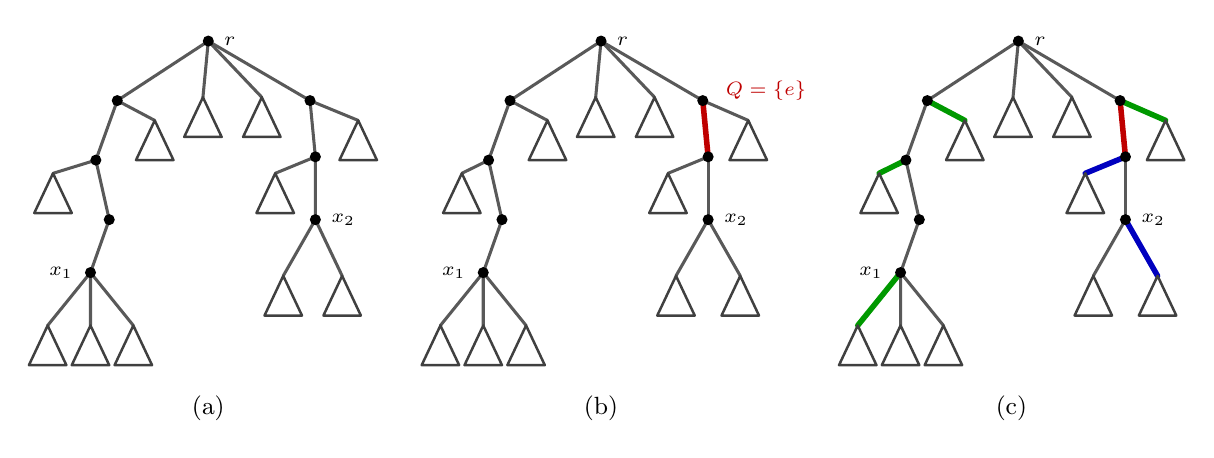
\begin{tikzpicture}[
        x=0.68cm,
        y=0.84cm,
        treeedge/.style={draw=black!65,line width=1.1pt,line cap=round},
        cutedge/.style={draw=green!60!black,line width=2pt,line cap=round},
        cutedgeblue/.style={draw=blue!75!black,line width=2pt,line cap=round},
        guessededge/.style={draw=red!75!black,line width=2pt,line cap=round},
        subtree/.style={draw=black!75,line width=0.9pt,line join=round},
    ]
        \coordinate (rOne) at (3.0,5.0);
        \coordinate (aOne) at (1.3,4.1);
        \coordinate (aTwo) at (0.9,3.2);
        \coordinate (aThree) at (1.15,2.3);
        \coordinate (xOne) at (0.8,1.5);
        \coordinate (bOne) at (4.9,4.1);
        \coordinate (bTwo) at (5.0,3.25);
        \coordinate (xTwo) at (5.0,2.3);
        \draw[treeedge] (rOne)--(aOne)--(aTwo)--(aThree)--(xOne);
        \draw[treeedge] (rOne)--(bOne)--(bTwo)--(xTwo);
        \draw[treeedge] (rOne)--(2.9,4.15) (rOne)--(4.0,4.15);
        \draw[subtree] (2.9,4.15)--(2.55,3.55)--(3.25,3.55)--cycle;
        \draw[subtree] (4.0,4.15)--(3.65,3.55)--(4.35,3.55)--cycle;
        \draw[treeedge] (aOne)--(2.0,3.8);
        \draw[subtree] (2.0,3.8)--(1.65,3.2)--(2.35,3.2)--cycle;
        \draw[treeedge] (aTwo)--(0.1,3.0);
        \draw[subtree] (0.1,3.0)--(-0.25,2.4)--(0.45,2.4)--cycle;
        \draw[treeedge] (bOne)--(5.8,3.8);
        \draw[subtree] (5.8,3.8)--(5.45,3.2)--(6.15,3.2)--cycle;
        \draw[treeedge] (bTwo)--(4.25,3.0);
        \draw[subtree] (4.25,3.0)--(3.9,2.4)--(4.6,2.4)--cycle;
        \draw[treeedge] (xOne)--(0.0,0.7) (xOne)--(0.8,0.7) (xOne)--(1.6,0.7);
        \draw[subtree] (0.0,0.7)--(-0.35,0.1)--(0.35,0.1)--cycle;
        \draw[subtree] (0.8,0.7)--(0.45,0.1)--(1.15,0.1)--cycle;
        \draw[subtree] (1.6,0.7)--(1.25,0.1)--(1.95,0.1)--cycle;
        \draw[treeedge] (xTwo)--(4.4,1.45) (xTwo)--(5.5,1.45);
        \draw[subtree] (4.4,1.45)--(4.05,0.85)--(4.75,0.85)--cycle;
        \draw[subtree] (5.5,1.45)--(5.15,0.85)--(5.85,0.85)--cycle;
        \foreach \p in {aOne,aTwo,aThree,bOne,bTwo} {\fill (\p) circle (2pt);}
        \foreach \p in {rOne,xOne,xTwo} {\fill (\p) circle (2pt);}
        \node[font=\scriptsize,anchor=west] at (3.12,5.0) {$r$};
        \node[font=\scriptsize,anchor=east] at (0.65,1.5) {$x_1$};
        \node[font=\scriptsize,anchor=west] at (5.12,2.3) {$x_2$};

        \begin{scope}[xshift=0.5cm]
        \coordinate (rTwo) at (9.6,5.0);
        \coordinate (cOne) at (7.9,4.1);
        \coordinate (cTwo) at (7.5,3.2);
        \coordinate (cThree) at (7.75,2.3);
        \coordinate (xOneTwo) at (7.4,1.5);
        \coordinate (dOne) at (11.5,4.1);
        \coordinate (dTwo) at (11.6,3.25);
        \coordinate (xTwoTwo) at (11.6,2.3);
        \draw[treeedge] (rTwo)--(cOne)--(cTwo)--(cThree)--(xOneTwo);
        \draw[treeedge] (rTwo)--(dOne);
        \draw[guessededge] (dOne)--(dTwo);
        \draw[treeedge] (dTwo)--(xTwoTwo);
        \draw[treeedge] (rTwo)--(9.5,4.15) (rTwo)--(10.6,4.15);
        \draw[subtree] (9.5,4.15)--(9.15,3.55)--(9.85,3.55)--cycle;
        \draw[subtree] (10.6,4.15)--(10.25,3.55)--(10.95,3.55)--cycle;
        \draw[treeedge] (cOne)--(8.6,3.8);
        \draw[subtree] (8.6,3.8)--(8.25,3.2)--(8.95,3.2)--cycle;
        \draw[treeedge] (cTwo)--(7.0,3.0);
        \draw[subtree] (7.0,3.0)--(6.65,2.4)--(7.35,2.4)--cycle;
        \draw[treeedge] (dOne)--(12.35,3.8);
        \draw[subtree] (12.35,3.8)--(12.0,3.2)--(12.7,3.2)--cycle;
        \draw[treeedge] (dTwo)--(10.85,3.0);
        \draw[subtree] (10.85,3.0)--(10.5,2.4)--(11.2,2.4)--cycle;
        \draw[treeedge] (xOneTwo)--(6.6,0.7) (xOneTwo)--(7.4,0.7) (xOneTwo)--(8.2,0.7);
        \draw[subtree] (6.6,0.7)--(6.25,0.1)--(6.95,0.1)--cycle;
        \draw[subtree] (7.4,0.7)--(7.05,0.1)--(7.75,0.1)--cycle;
        \draw[subtree] (8.2,0.7)--(7.85,0.1)--(8.55,0.1)--cycle;
        \draw[treeedge] (xTwoTwo)--(11.0,1.45) (xTwoTwo)--(12.2,1.45);
        \draw[subtree] (11.0,1.45)--(10.65,0.85)--(11.35,0.85)--cycle;
        \draw[subtree] (12.2,1.45)--(11.85,0.85)--(12.55,0.85)--cycle;
        \foreach \p in {cOne,cTwo,cThree,dOne,dTwo} {\fill (\p) circle (2pt);}
        \foreach \p in {rTwo,xOneTwo,xTwoTwo} {\fill (\p) circle (2pt);}
        \node[font=\scriptsize,anchor=west] at (9.72,5.0) {$r$};
        \node[font=\scriptsize,anchor=east] at (7.25,1.5) {$x_1$};
        \node[font=\scriptsize,anchor=west] at (11.72,2.3) {$x_2$};
        \node[font=\scriptsize,text=red!75!black,anchor=west] at (11.75,4.25) {$Q=\{e\}$};
        \end{scope}

        \begin{scope}[xshift=5.8cm]
        \coordinate (rThree) at (9.6,5.0);
        \coordinate (cOneThree) at (7.9,4.1);
        \coordinate (cTwoThree) at (7.5,3.2);
        \coordinate (cThreeThree) at (7.75,2.3);
        \coordinate (xOneThree) at (7.4,1.5);
        \coordinate (dOneThree) at (11.5,4.1);
        \coordinate (dTwoThree) at (11.6,3.25);
        \coordinate (xTwoThree) at (11.6,2.3);
        \draw[treeedge] (rThree)--(cOneThree)--(cTwoThree)--(cThreeThree)--(xOneThree);
        \draw[treeedge] (rThree)--(dOneThree);
        \draw[treeedge] (dOneThree)--(dTwoThree);
        \draw[guessededge] (dOneThree)--(dTwoThree);
        \draw[treeedge] (dTwoThree)--(xTwoThree);
        \draw[treeedge] (rThree)--(9.5,4.15) (rThree)--(10.6,4.15);
        \draw[subtree] (9.5,4.15)--(9.15,3.55)--(9.85,3.55)--cycle;
        \draw[subtree] (10.6,4.15)--(10.25,3.55)--(10.95,3.55)--cycle;
        \draw[treeedge] (cOneThree)--(8.6,3.8);
        \draw[cutedge] (cOneThree)--(8.6,3.8);
        \draw[subtree] (8.6,3.8)--(8.25,3.2)--(8.95,3.2)--cycle;
        \draw[treeedge] (cTwoThree)--(7.0,3.0);
        \draw[cutedge] (cTwoThree)--(7.0,3.0);
        \draw[subtree] (7.0,3.0)--(6.65,2.4)--(7.35,2.4)--cycle;
        \draw[treeedge] (dOneThree)--(12.35,3.8);
        \draw[cutedge] (dOneThree)--(12.35,3.8);
        \draw[subtree] (12.35,3.8)--(12.0,3.2)--(12.7,3.2)--cycle;
        \draw[treeedge] (dTwoThree)--(10.85,3.0);
        \draw[cutedgeblue] (dTwoThree)--(10.85,3.0);
        \draw[subtree] (10.85,3.0)--(10.5,2.4)--(11.2,2.4)--cycle;
        \draw[treeedge] (xOneThree)--(6.6,0.7);
        \draw[cutedge] (xOneThree)--(6.6,0.7);
        \draw[treeedge] (xOneThree)--(7.4,0.7) (xOneThree)--(8.2,0.7);
        \draw[subtree] (6.6,0.7)--(6.25,0.1)--(6.95,0.1)--cycle;
        \draw[subtree] (7.4,0.7)--(7.05,0.1)--(7.75,0.1)--cycle;
        \draw[subtree] (8.2,0.7)--(7.85,0.1)--(8.55,0.1)--cycle;
        \draw[treeedge] (xTwoThree)--(11.0,1.45) (xTwoThree)--(12.2,1.45);
        \draw[cutedgeblue] (xTwoThree)--(12.2,1.45);
        \draw[subtree] (11.0,1.45)--(10.65,0.85)--(11.35,0.85)--cycle;
        \draw[subtree] (12.2,1.45)--(11.85,0.85)--(12.55,0.85)--cycle;
        \foreach \p in {cOneThree,cTwoThree,cThreeThree,dOneThree,dTwoThree} {\fill (\p) circle (2pt);}
        \fill (rThree) circle (2pt);
        \fill (xOneThree) circle (2pt);
        \fill (xTwoThree) circle (2pt);
        \node[font=\scriptsize,anchor=west] at (9.72,5.0) {$r$};
        \node[font=\scriptsize,anchor=east] at (7.25,1.5) {$x_1$};
        \node[font=\scriptsize,anchor=west] at (11.72,2.3) {$x_2$};
        \end{scope}
        \node[font=\small] at (3.0,-0.55) {(a)};
        \node[font=\small,xshift=0.5cm] at (9.6,-0.55) {(b)};
        \node[font=\small] at (18.0,-0.55) {(c)};
    \end{tikzpicture}
    \caption{(a) The initial tree with centroids $r$, $x_1$ and $x_2$. (b) The guess $Q=\brc{e}$ (red dashed). (c) Green edges are cuts in the component containing $x_1$, blue edges are cuts in the component containing $x_2$, and the guessed edge $e$ remains red and dashed.}
    \label{fig:three-centroid-coverage}
    \end{figure}
